\section{Introduktion}

%\subsection{Ern\"{o} Rubik}
\begin{frame}{Ern\"{o} Rubik}
\begin{itemize}
	\item<1>F\o{}dt i Ungarn i 1944
	\item<1>Ingeni\o{}r med speciale i arkitektur
	\item Patent i 1977
	\item Varem\ae{}rke
\end{itemize}
\begin{figure}
	\centering
		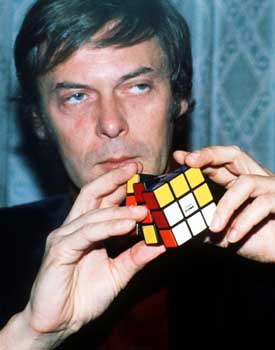
\includegraphics[width=0.35\textwidth]{input/pics/ErnoRubik.jpg}
	\label{fig:ErnoRubik}
\end{figure}

\end{frame}

%\subsection{Rubik's Terningen}
\begin{frame}{Rubik's Terningen}
\begin{itemize}
	\item<1>26 cubies
	\item<1>6 faces	
	\begin{itemize}
		\item<1>9 facelets pr. face
	\end{itemize}
\end{itemize}
\begin{figure}[bp]
	\centering
		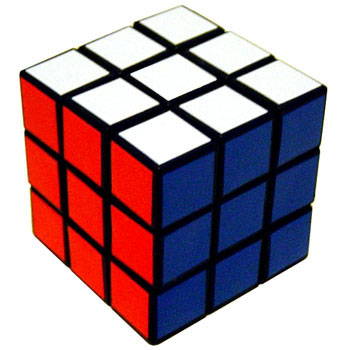
\includegraphics[scale=0.25]{input/pics/rubiks-cube.jpg}
	%\caption{En l�st Rubik's terning}
	\label{fig:rubiks-cube}
\end{figure}

\end{frame}